\documentclass{article}
\title{Backgammon-specification}
\usepackage[fencedCode]{markdown}
\usepackage{graphicx}
\usepackage[export]{adjustbox}
\usepackage{xcolor}
\usepackage{fvextra}
\DefineVerbatimEnvironment{Highlighting}{Verbatim}
  {breaklines,breakanywhere,commandchars=\\\{\}}
\fvset{breaklines}
\title{Backgammon++ specification}
\usepackage{geometry}
 \geometry{
 a4paper,
 total={170mm,257mm},
 left=20mm,
 top=20mm,
 }
\begin{document}
\maketitle

\section{Game summary}

Backgammon is a strategic game that includes dice rolls and moving tokens across the board.
The game lasts until one of the players moves all of their tokens to the goal. Games can be
played between bots and/or human players. A played match can be saved for later analysis.

\section{UML diagrams}

\section{Use case diagram}

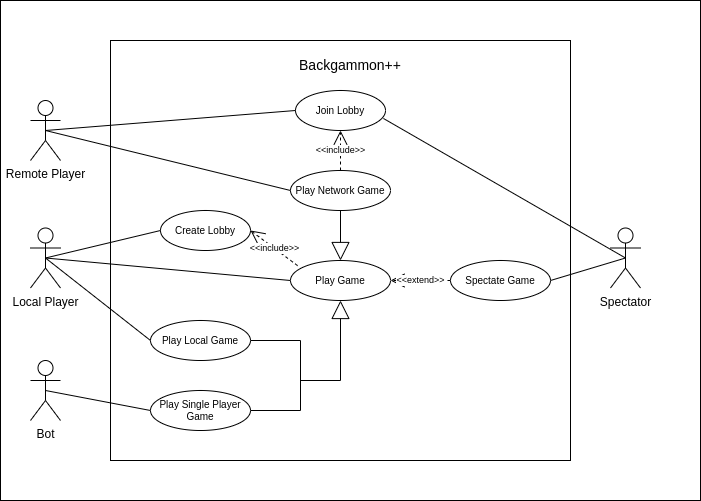
\includegraphics[max size={\textwidth}{\textheight}]{UseCaseDiagram.png}
\clearpage

\section{Sequence diagrams}

\markdownInput{UseCase_CreateLobby.md}
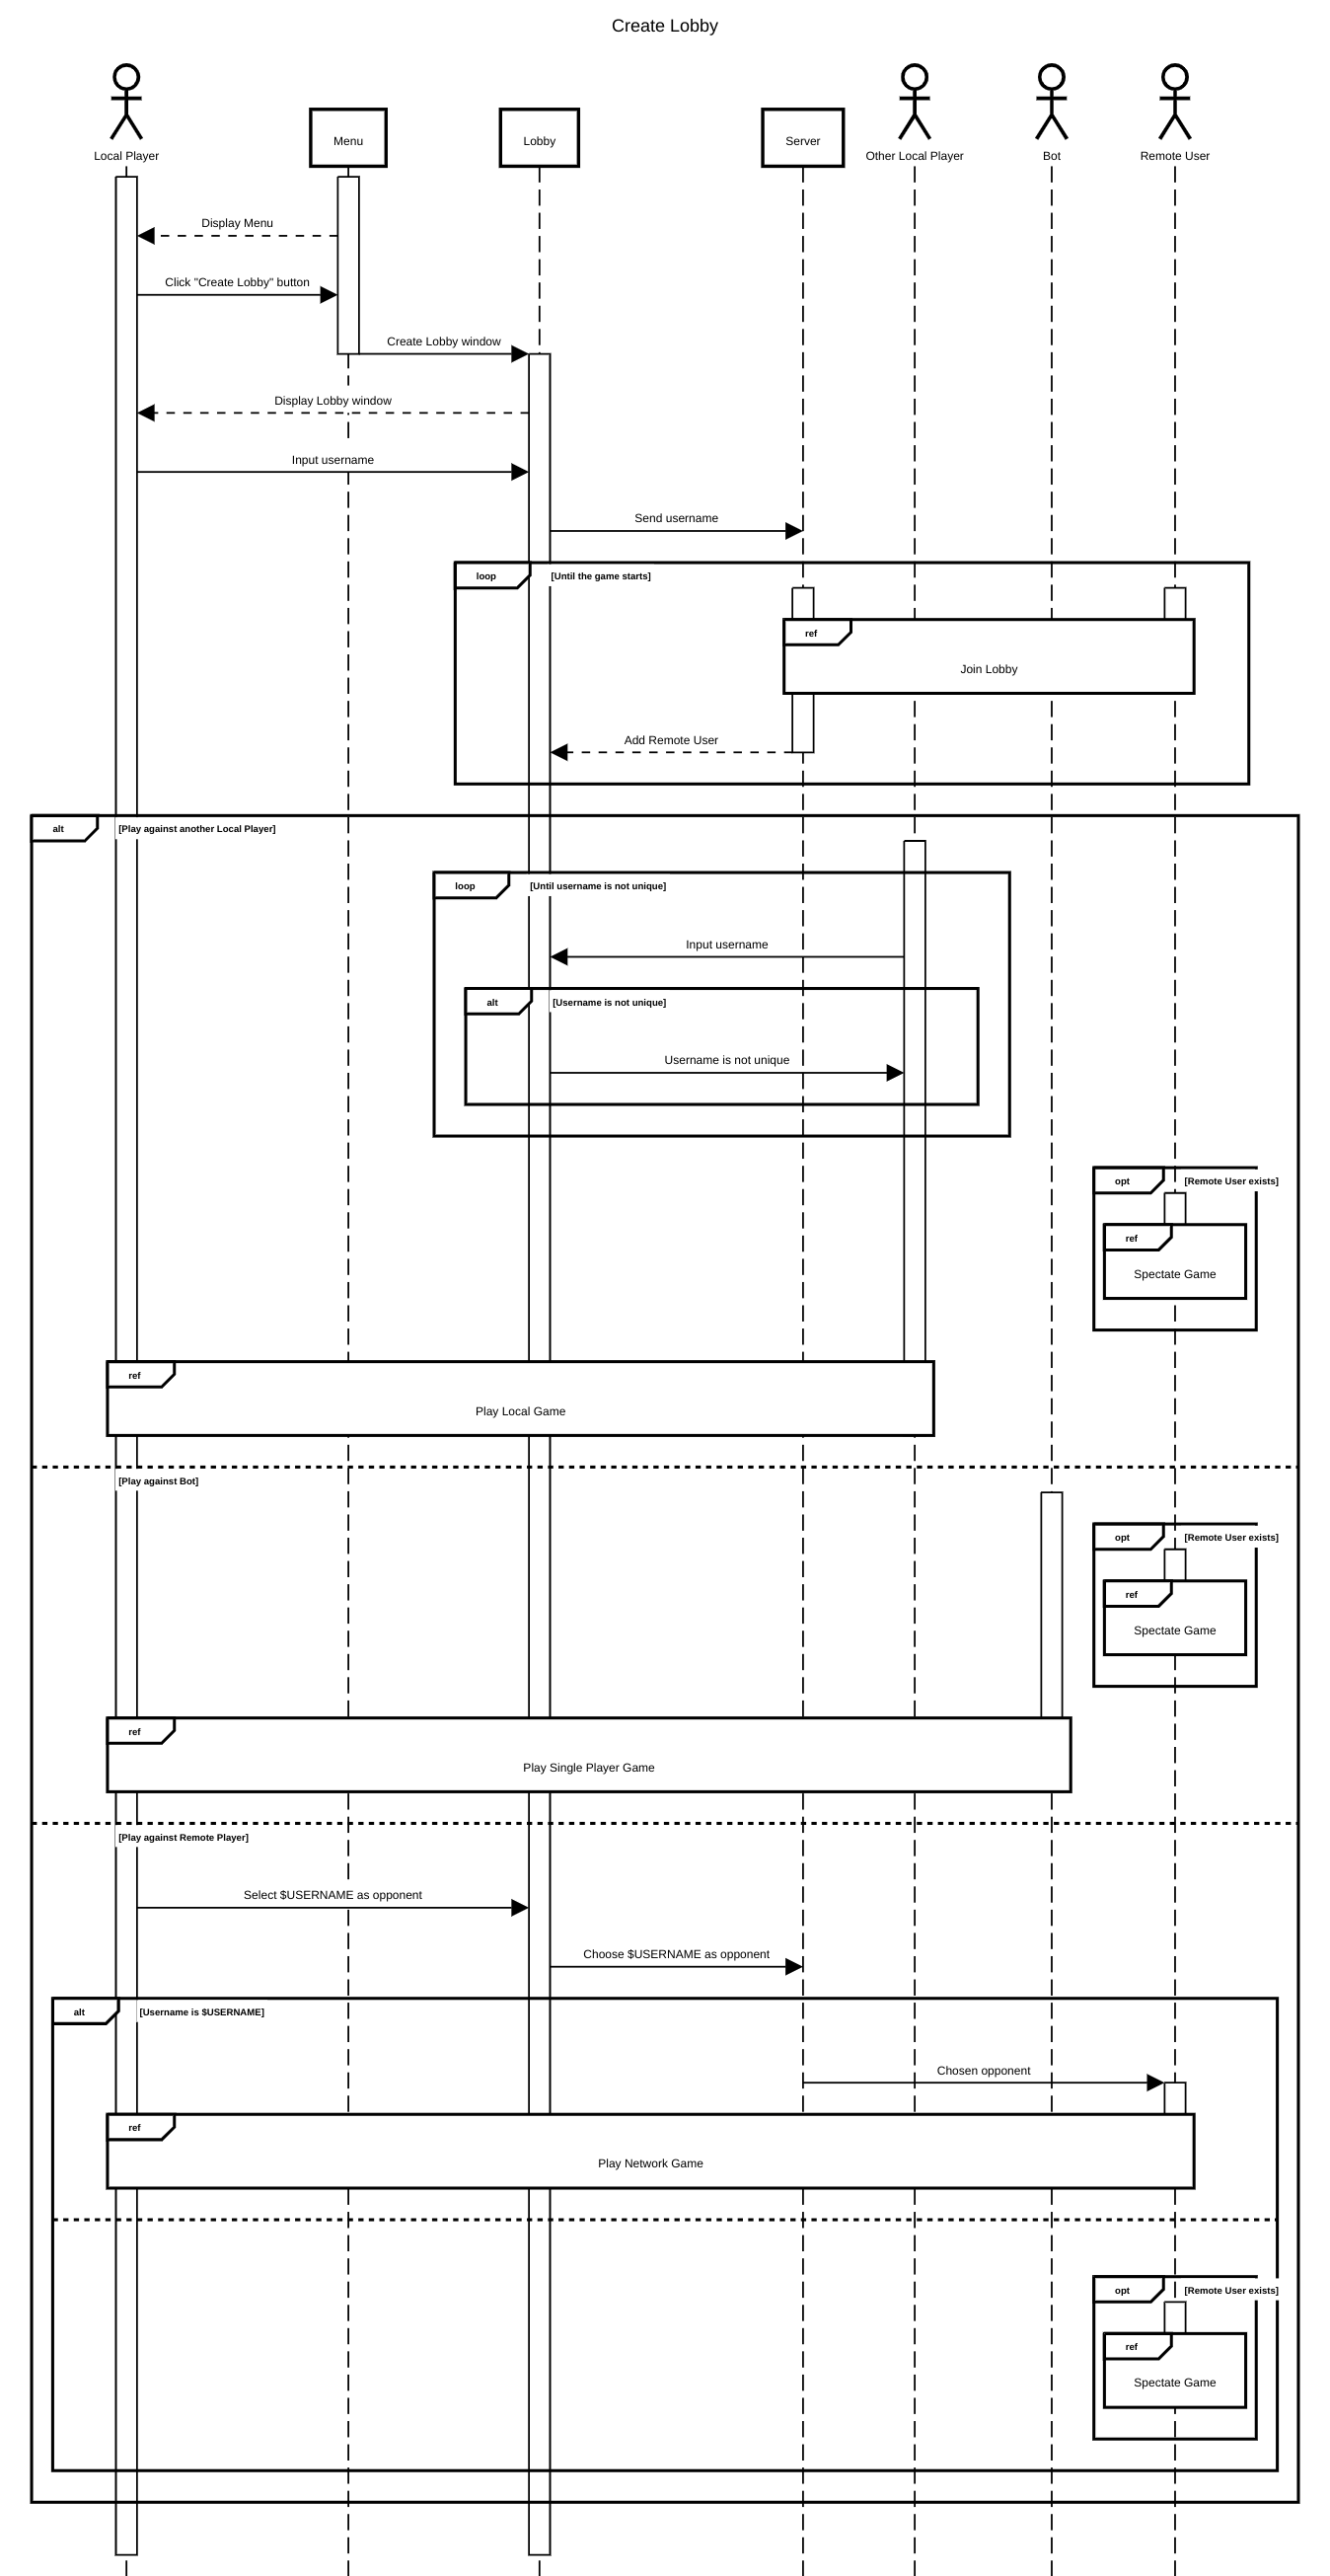
\includegraphics[max size={\textwidth}{\textheight}]{SequenceDiagram_CreateLobby.png}
\clearpage

\markdownInput{UseCase_JoinLobby.md}
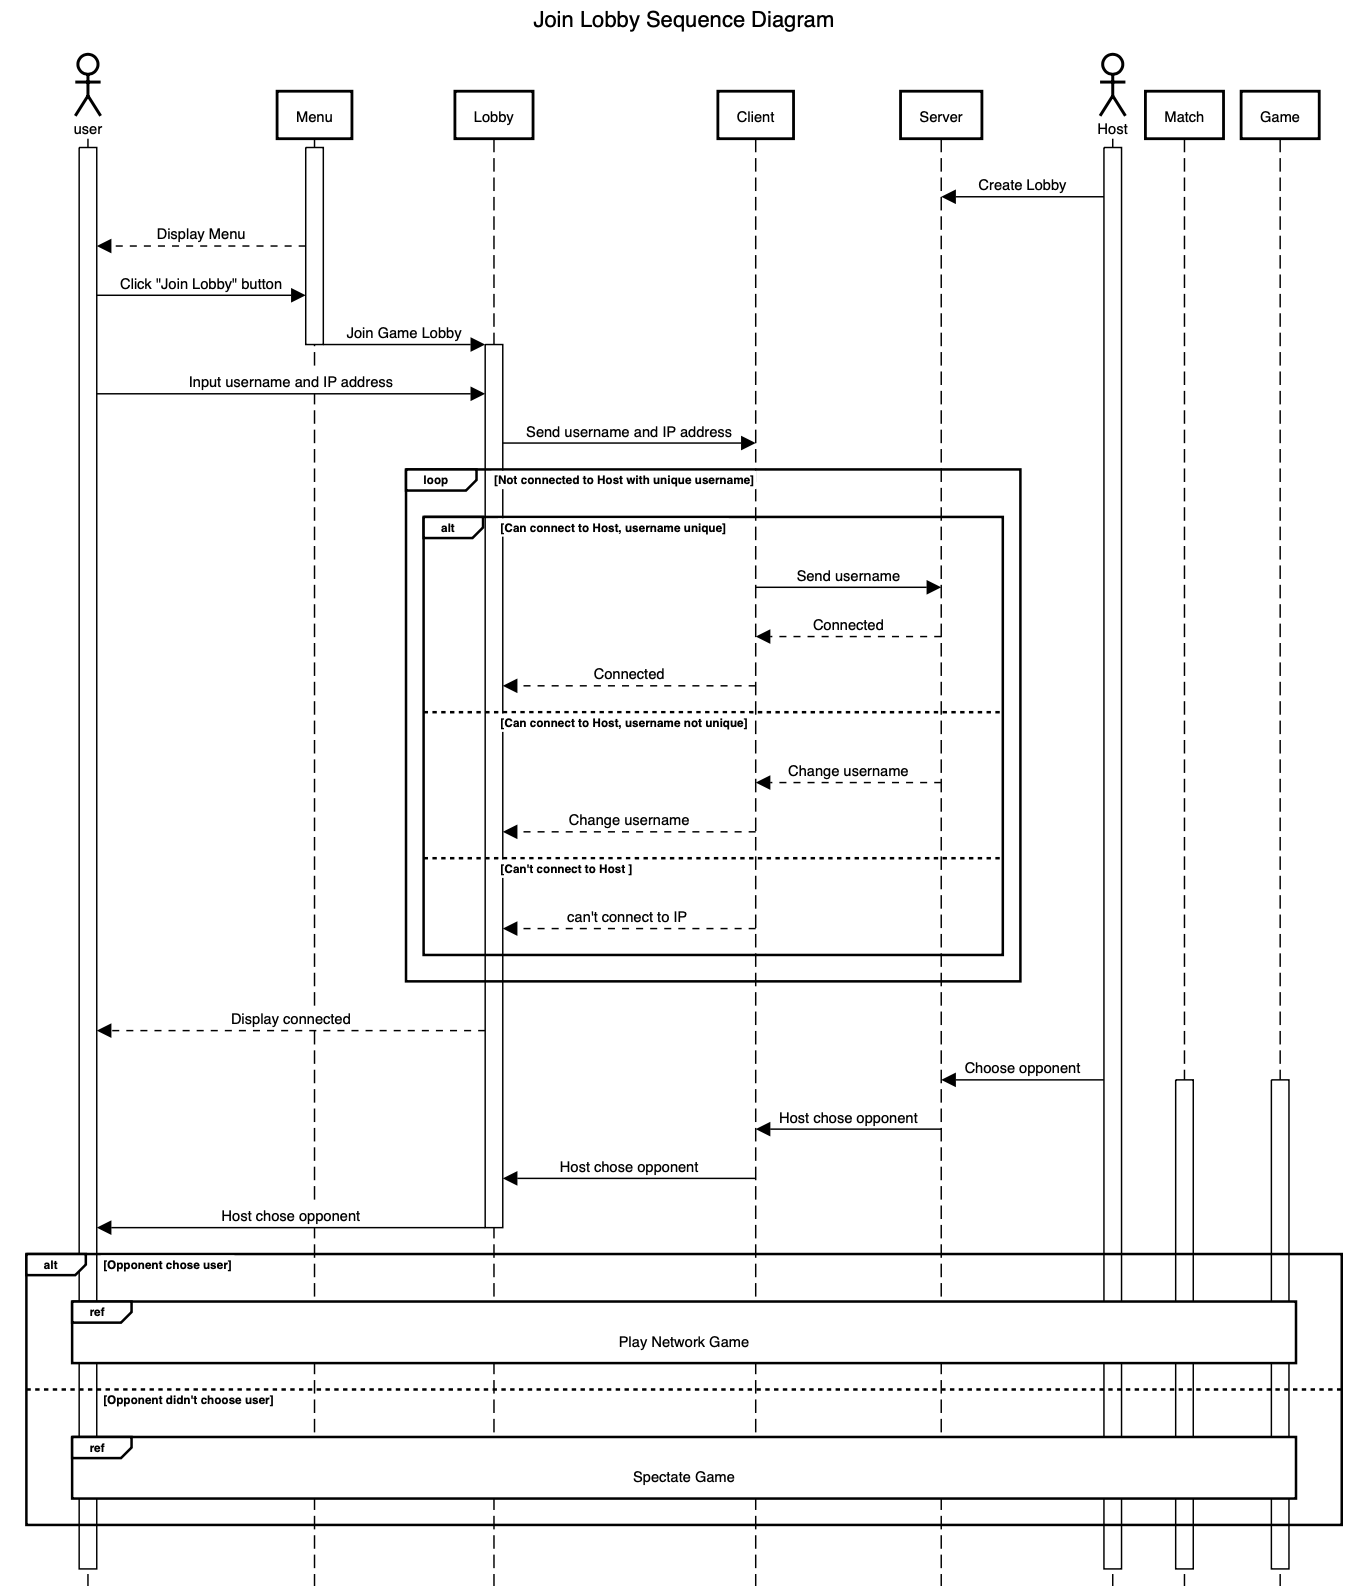
\includegraphics[max size={\textwidth}{\textheight}]{SequenceDiagram_JoinLobby.png}
\clearpage

\markdownInput{UseCase_PlayGame.md}
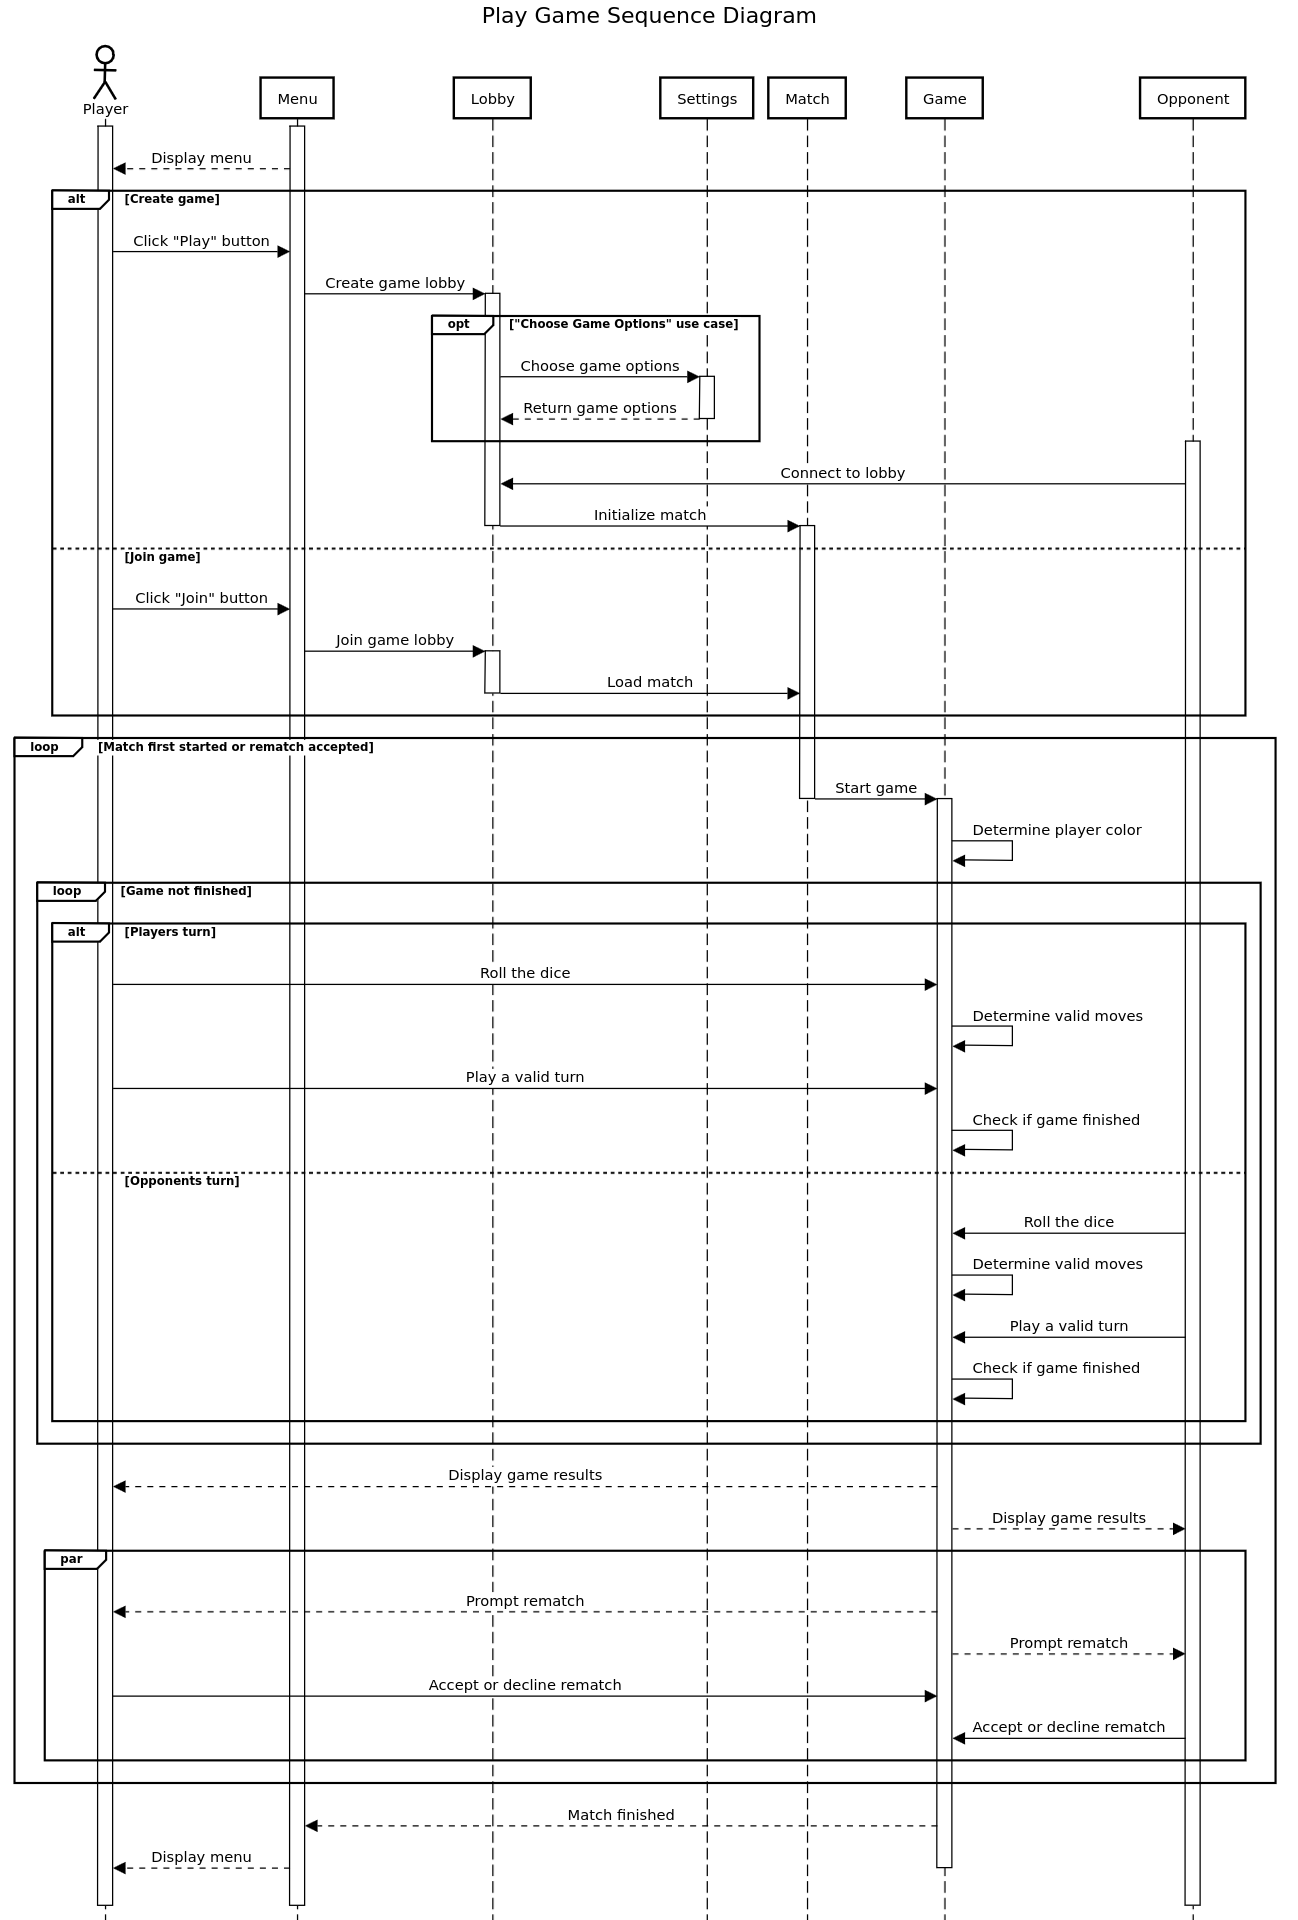
\includegraphics[max size={\textwidth}{\textheight}]{SequenceDiagram_PlayGame.png}
\clearpage

\markdownInput{UseCase_PlaySinglePlayerMatch.md}
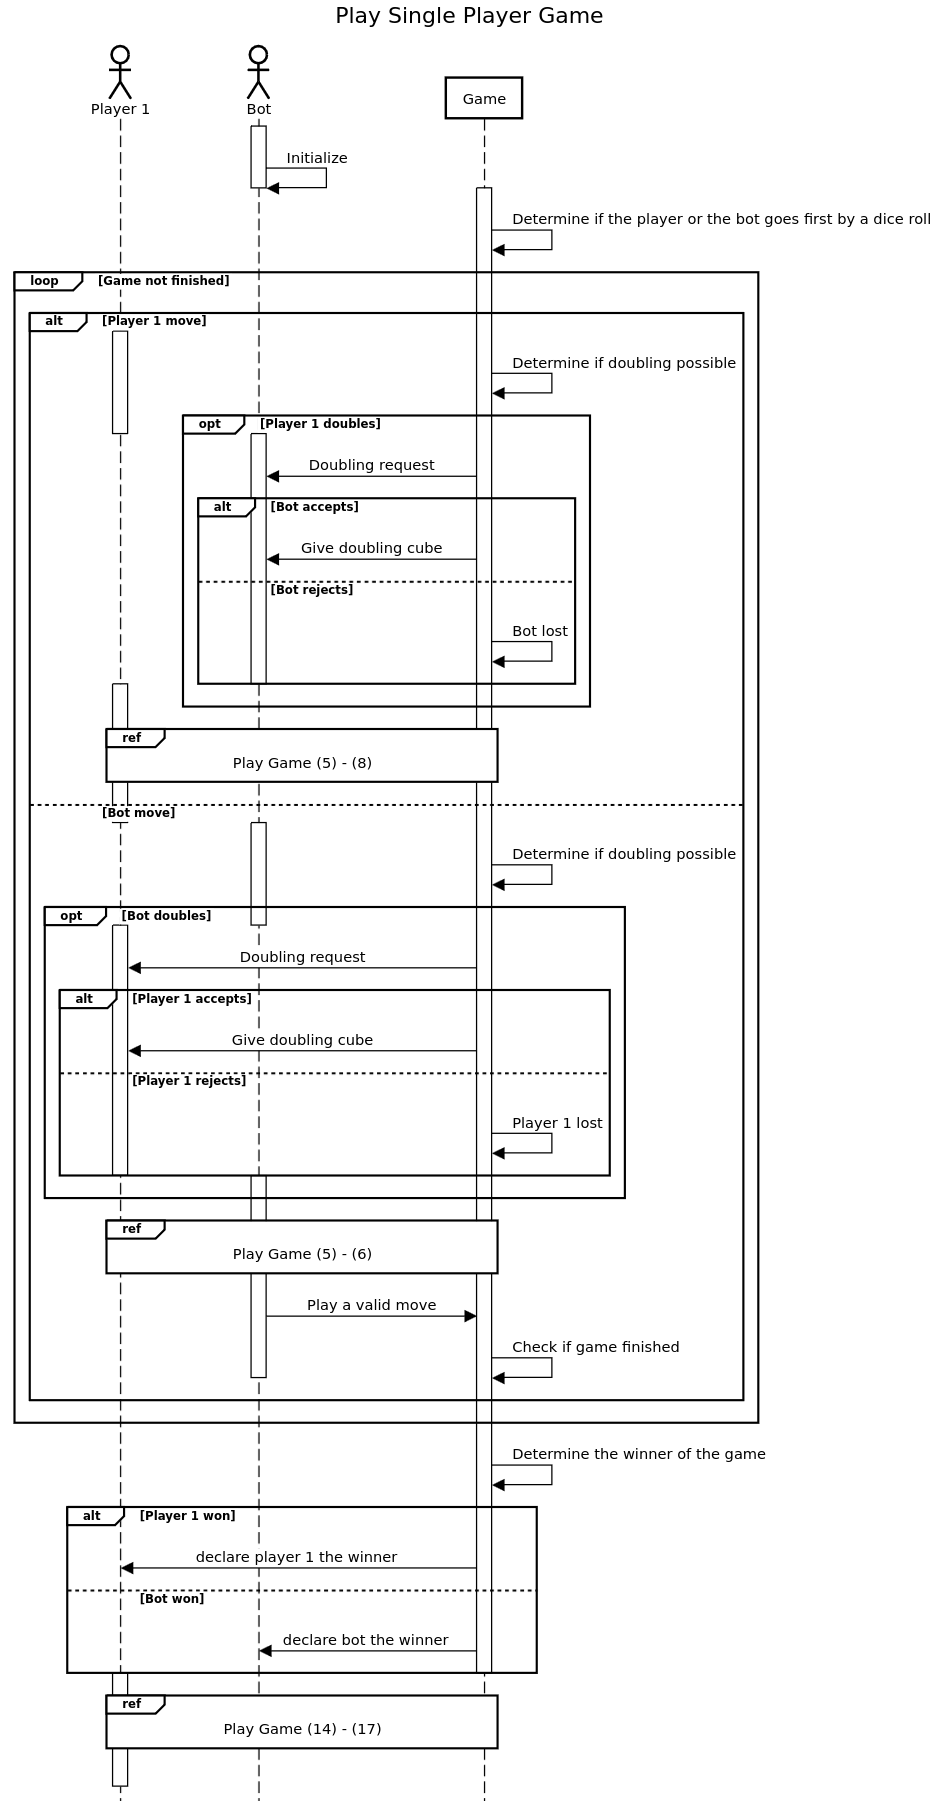
\includegraphics[max size={\textwidth}{\textheight}]{SequenceDiagram_PlaySinglePlayerGame.png}
\clearpage

\markdownInput{UseCase_PlayLocalGame.md}
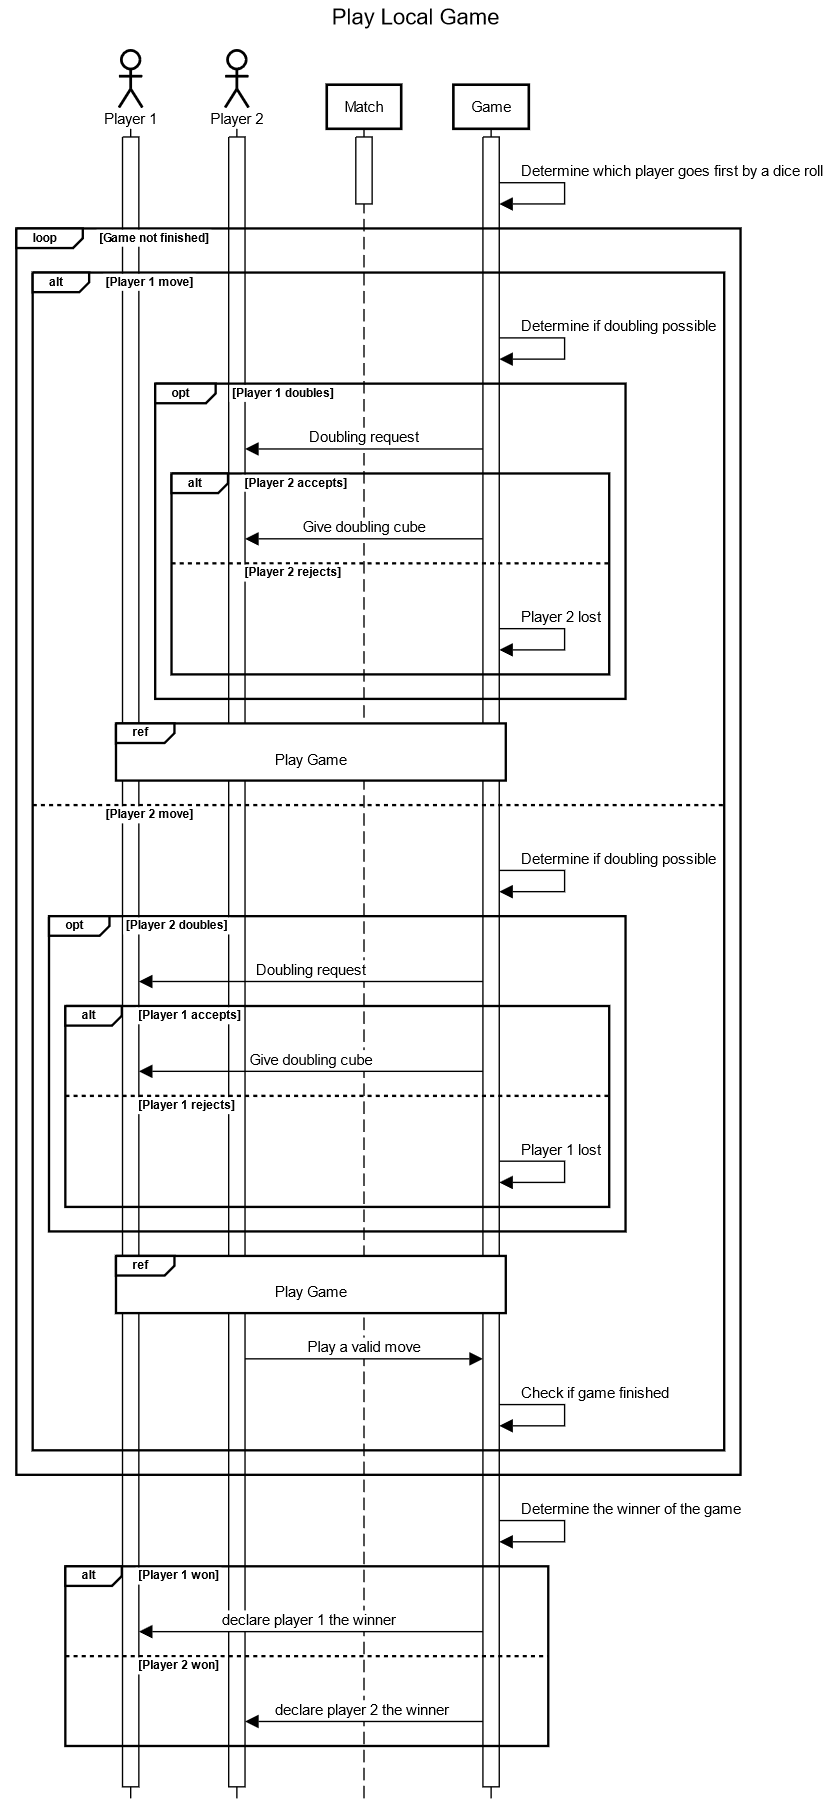
\includegraphics[max size={\textwidth}{\textheight}]{SequenceDiagram_PlayLocalGame.png}
\clearpage

\markdownInput{UseCase_PlayNetworkGame.md}
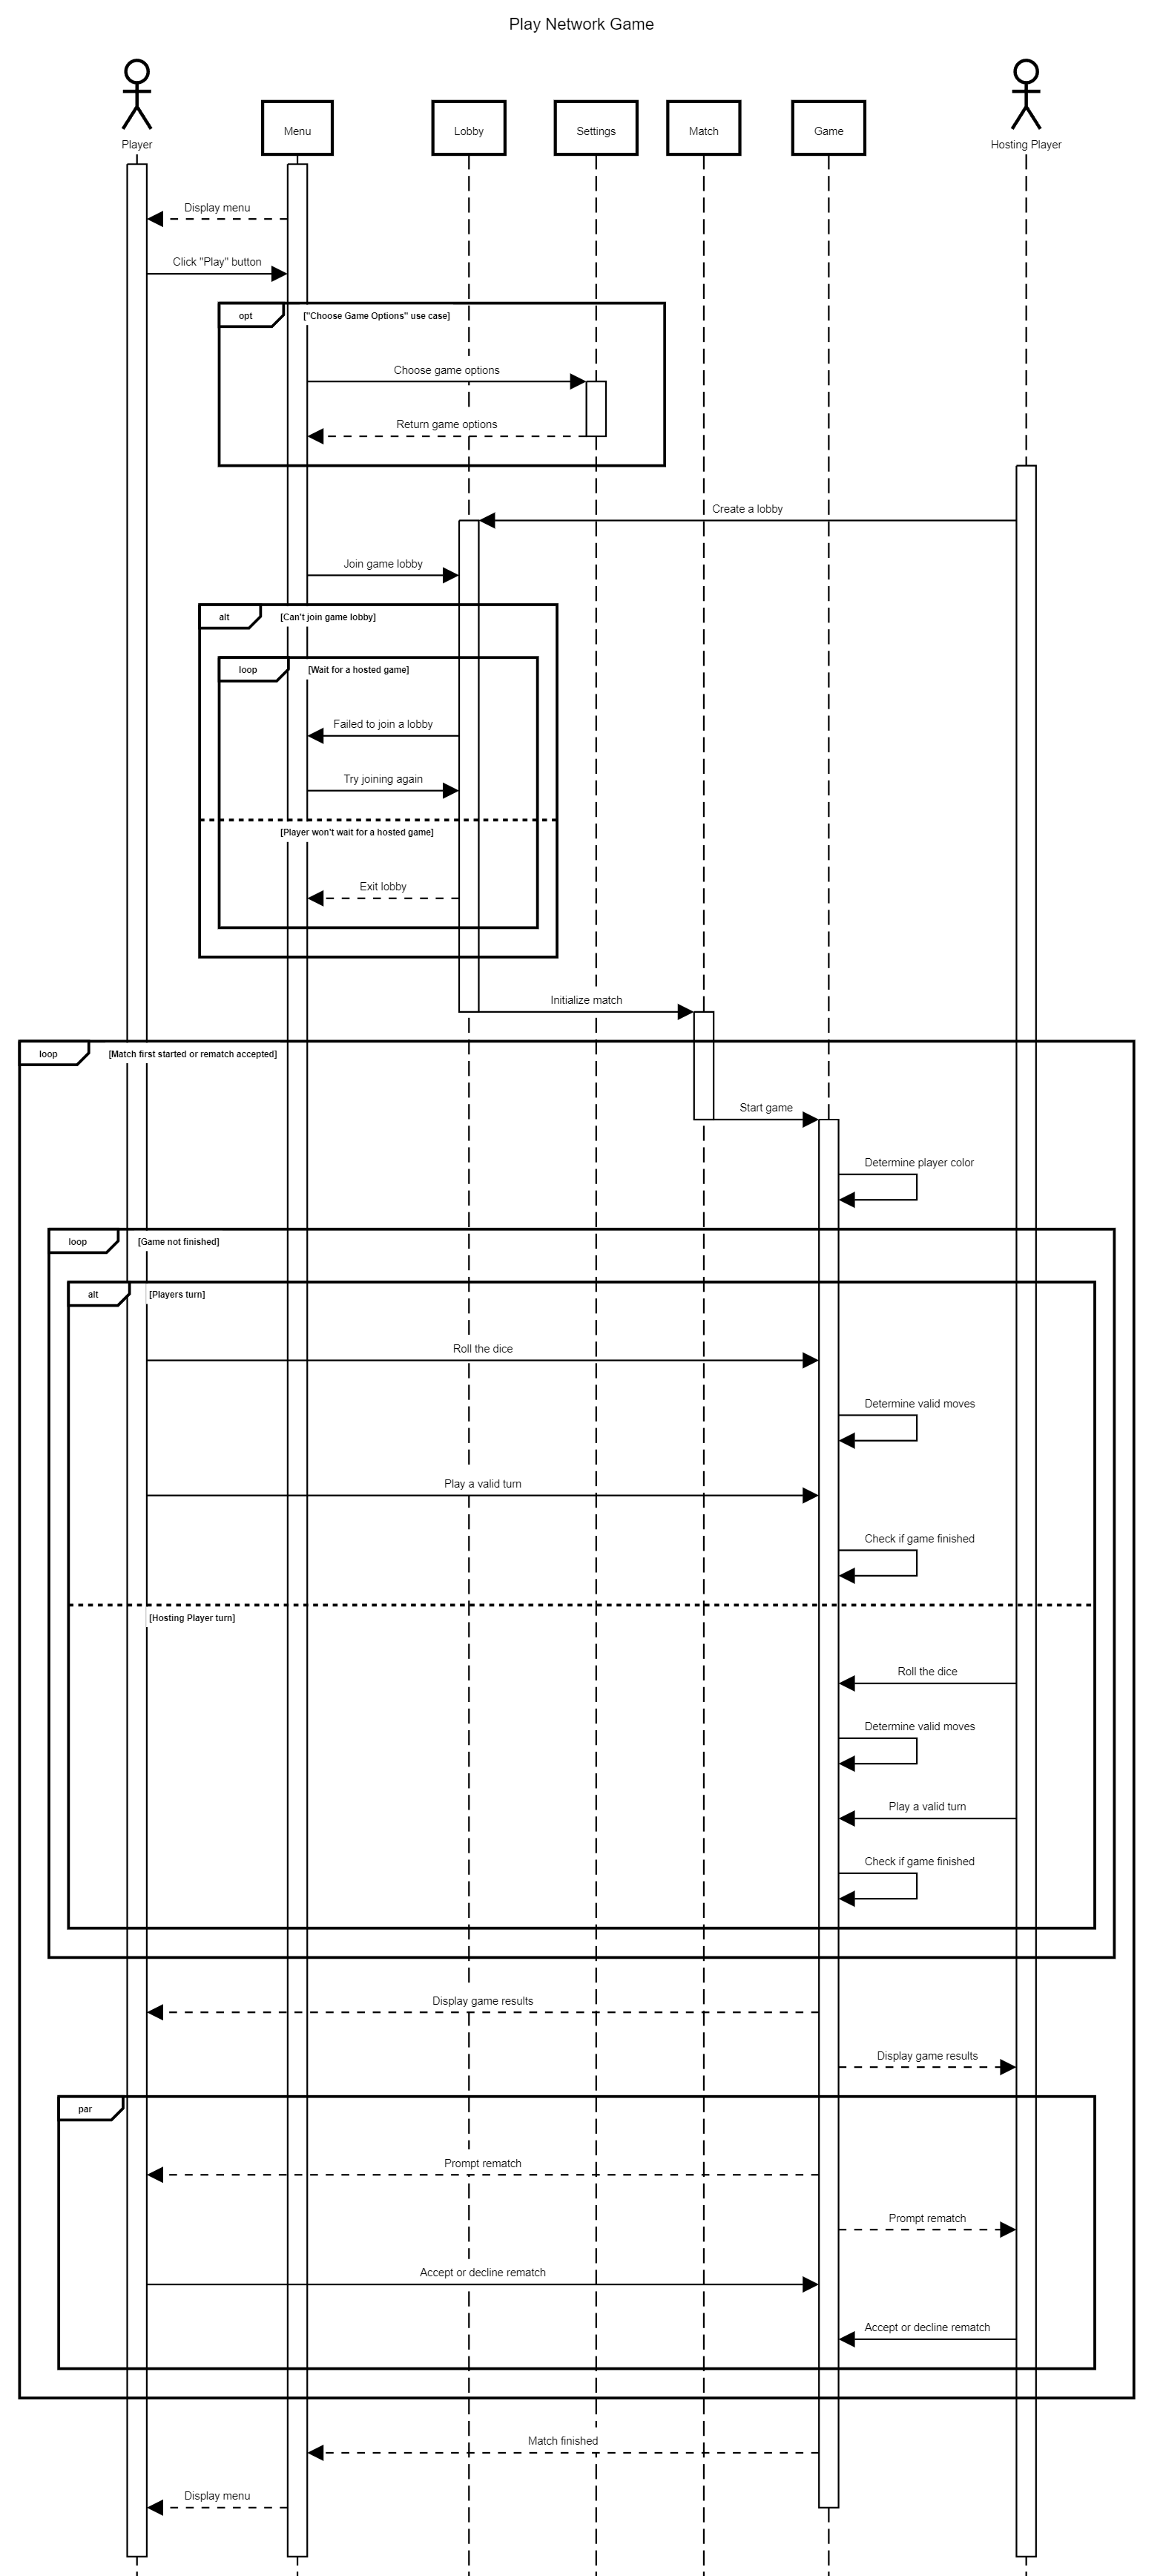
\includegraphics[max size={\textwidth}{\textheight}]{SequenceDiagram_PlayNetworkGame.png}
\clearpage

\markdownInput{UseCase_SpectateGame.md}
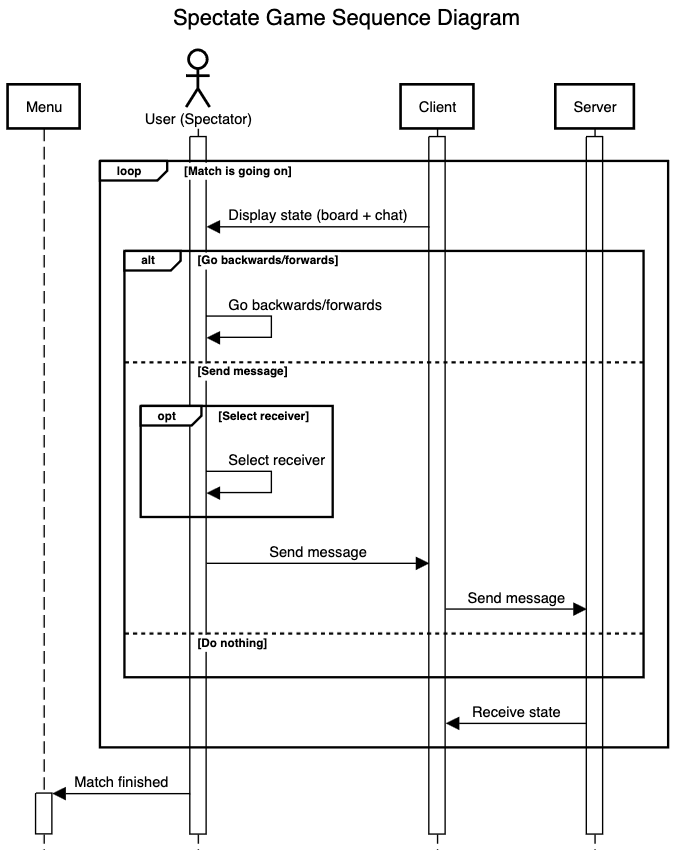
\includegraphics[max size={\textwidth}{\textheight}]{SequenceDiagram_SpectateGame.png}
\clearpage

\section{Class diagram}
\noindent\makebox[\textwidth]{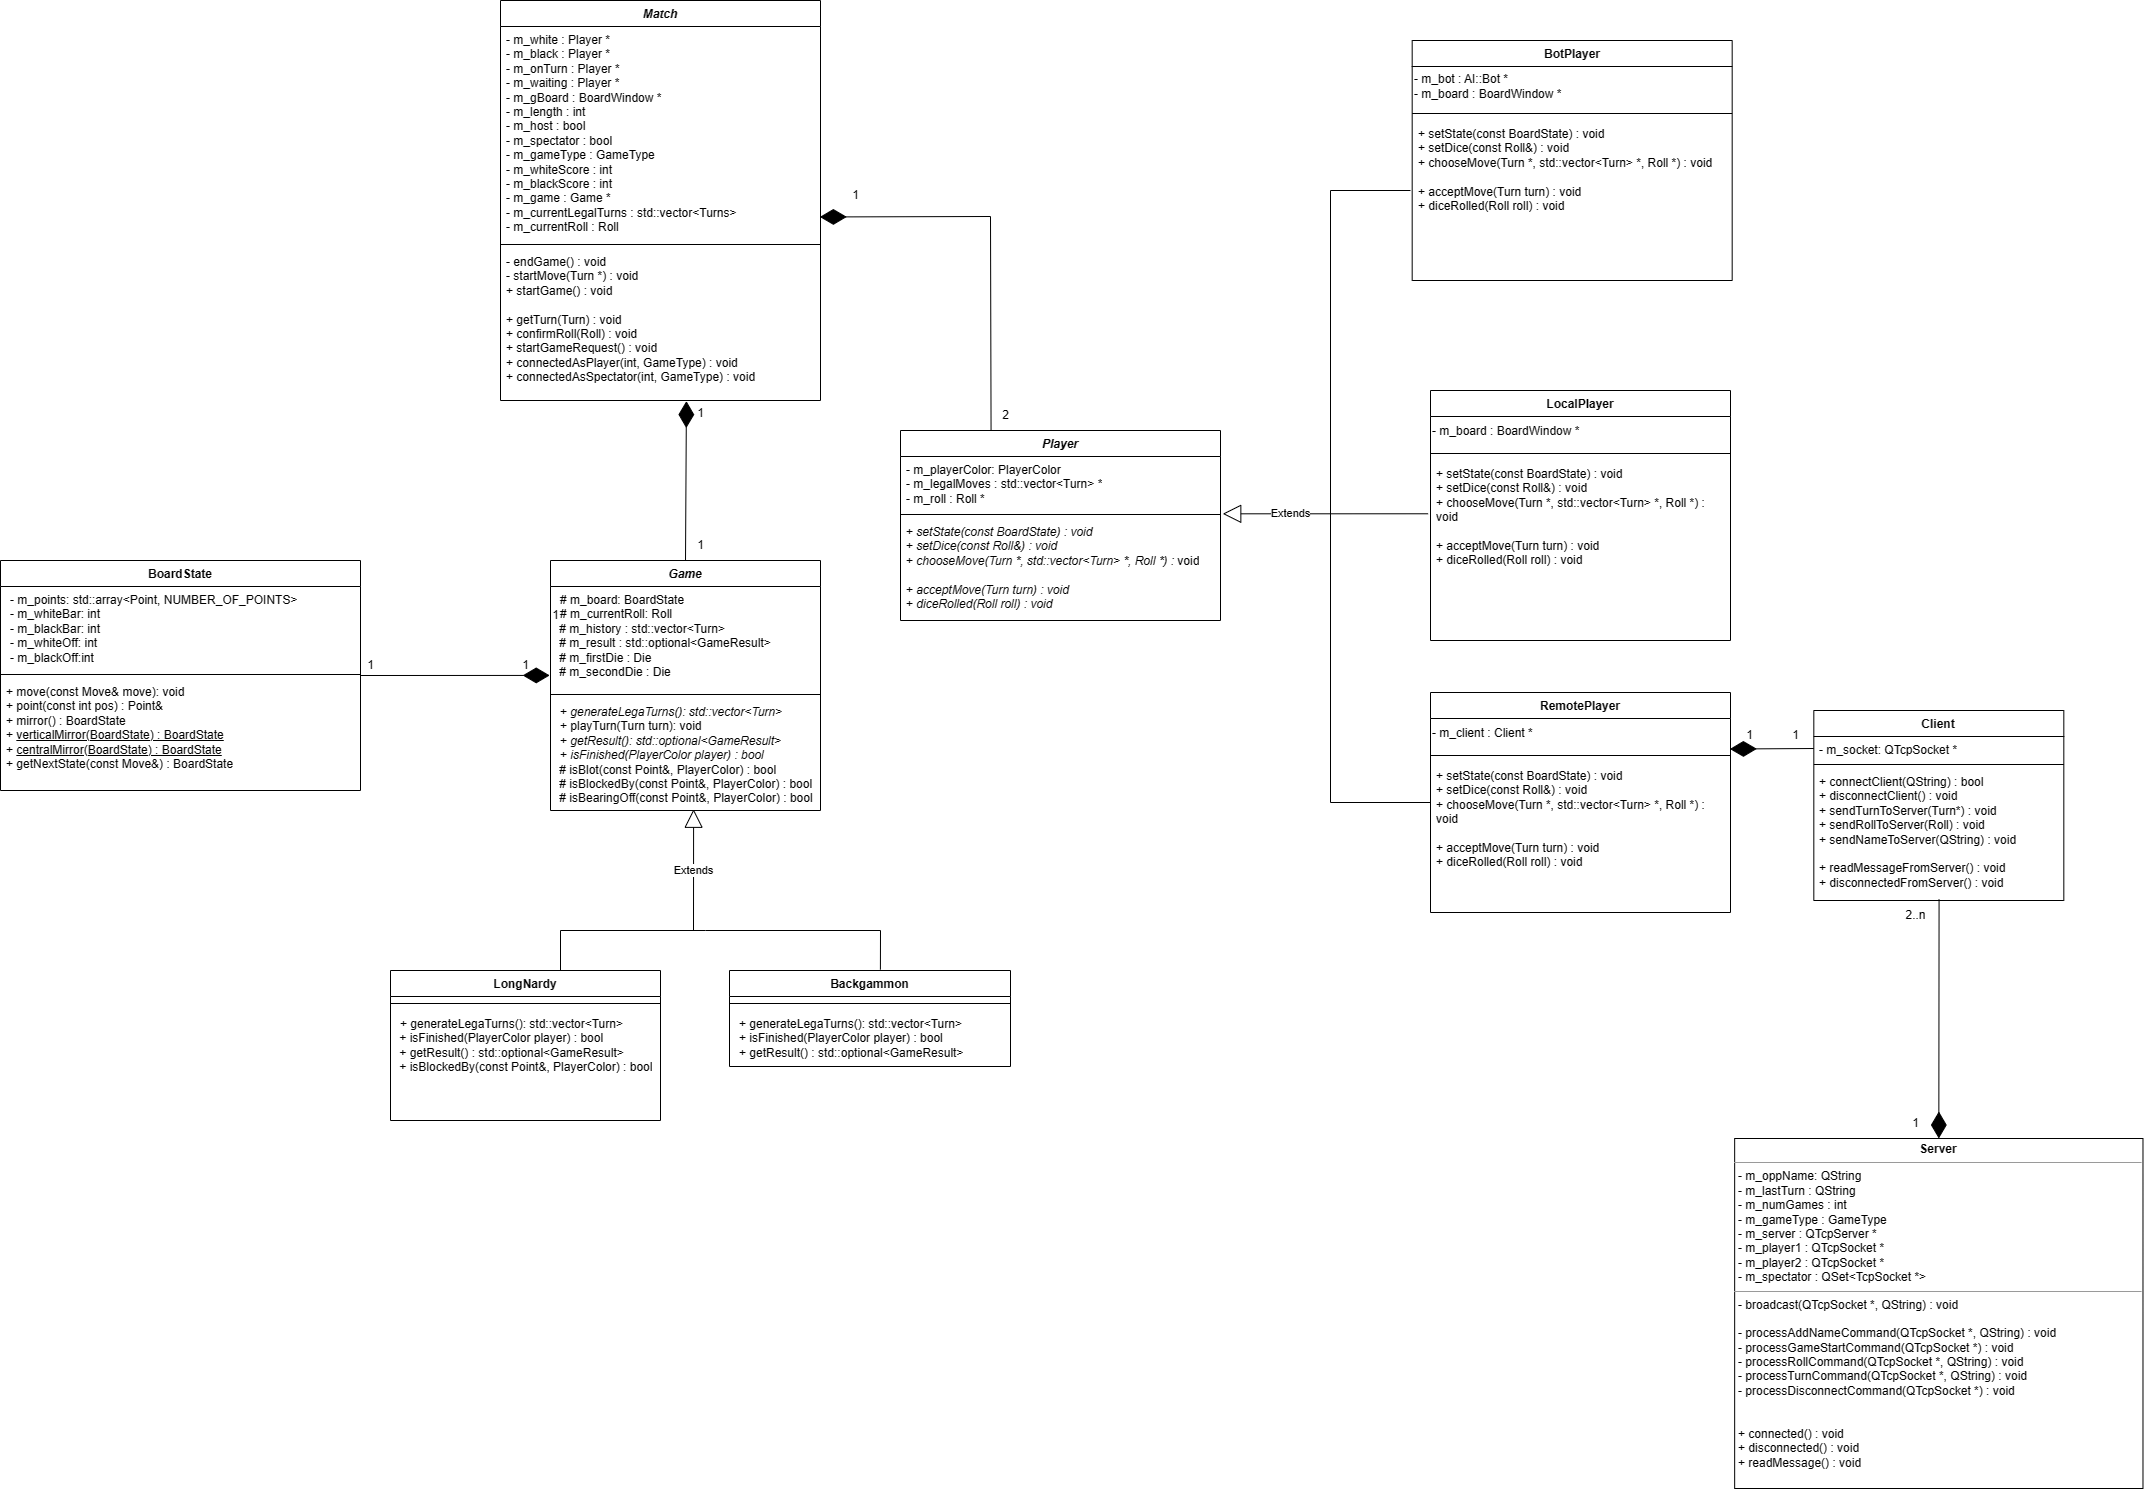
\includegraphics[width=\paperwidth]{ClassDiagram.png}}

\end{document}
